\RequirePackage{fix-cm} % Added by the template.

% smallextended below is the one used by MPC,  see:
% https://www.springer.com/journal/12532/submission-guidelines
\documentclass[smallextended]{svjour3}       % onecolumn (second format)
%\usepackage[brazil]{babel}
\usepackage[utf8]{inputenc}
\usepackage{float}
\usepackage{url}
\usepackage{amssymb}
%\usepackage{amsthm}
\usepackage{amsmath}
\usepackage{listings}
\usepackage{graphicx}
\usepackage{xcolor}
\usepackage{hyphenat}
\usepackage{verbatim}
%\usepackage{cleveref} % Cannot be used with svjour3
\usepackage{hyperref} % For autoref
\usepackage{seqsplit} % To allow breaks inside texttt
\usepackage[hmargin=3cm,vmargin=3cm]{geometry}

\usepackage[normalem]{ulem} % for \sout
\usepackage{tikz}

\newif\iffinalversion
\newcommand{\newtext}[1]{\iffinalversion%
#1%
\else%
\textcolor{blue}{#1}%
\fi%
}
\newcommand{\oldtext}[1]{\iffinalversion%
#1%
\else%
\textcolor{red}{\sout{#1}}%
\fi%
}

\newcommand{\mytilde}{\raise.17ex\hbox{$\scriptstyle\mathtt{\sim}$}}

\setlength\parindent{0pt}

\newcommand{\isep}{\mathrel{{.}\,{.}}\nobreak} % for integer ranges
\newcommand{\inlinecode}[1]{\texttt{\seqsplit{#1}}}

\makeatletter
\newcommand\gobblepars{%
    \@ifnextchar\par%
        {\expandafter\gobblepars\@gobble}%
        {}}
\makeatother

\newcounter{concern}
\newenvironment{concern}{%
    \refstepcounter{concern}\par\smallskip\noindent%
    \textbf{Concern~\#\theconcern}: ``\itshape\gobblepars}%
    {\unskip''\smallskip}
\newcommand{\concernautorefname}{Concern}

\newcounter{answer}
\newenvironment{answer}{%
    \refstepcounter{answer}\par\smallskip\noindent%
    \textbf{Our answer}: \gobblepars}%
    {\unskip\bigskip}
\newcommand{\answerautorefname}{Answer}

\begin{document}
\pagestyle{empty}

\vspace{2cm}

\begin{flushright}
   \begin{minipage}{7cm}
      Henrique Becker \\
      Instituto de Informática - UFRGS \\
      Av. Bento Gonçalves, 9500. \\
      91501-970 Porto Alegre - RS - Brazil \\
      E-mail: hbecker@inf.ufrgs.br \\
   \end{minipage}
\end{flushright}

\begin{flushleft}
%November, 24$^{\text{th}}$ 2016.
%December, 06$^{\text{th}}$ 2018.
\today

\vspace{1.5cm}

Dear Sanjeeb Dash,\\
Area Editor of Mathematical Programming Computation
\end{flushleft}

\bigskip
First of all, we would like to thank all reviewers for their comments on our paper ``Enhanced Formulation for Guillotine 2D Cutting Problems''.
We would also like to thank the editor for giving the opportunity of sending a revised version of the paper for possible publication in the Mathematical Programming Computation.
We have addressed all the questions and issues raised by the reviewers and the editor, which we discuss in the report enclosed below.
For the convenience of the reviewers, their questions and requests are quoted, numbered and italicized, and excerpts from the revised paper which address the request are colored in blue and quoted.

\bigskip

\begin{flushleft}
Yours Sincerely,\\
Henrique Becker (on behalf of all authors)
\end{flushleft}

\newpage

\section{Area Editor}

% NOTE: \label needs to be touching the last non-space character of the
% concern, otherwise a space is inserted between the text and the closing
% quotes.
\begin{concern}
I also recommend that the authors try to justify a bit more why the guillotine cutting version is important (e.g. are most of the 2-d cutting stock problems based on guillotine cuts in practice?)\label{con:justify_problem_importance}
\end{concern}

\begin{answer}
The first paragraph of motivation was rewritten to include a justification of the importance of guillotine cuts. The rewritten paragraph follows:\\
\newtext{Guillotine cutting problems of interest of the industry, especially the wood\cite{yanasse:linear:2008,morabito:hardboard:2007} and glass cutting industries\cite{clautiaux:2019,parreno:2020}, often because of machinery limitations. The cutting optimization problem proposed in the \emph{ROADEF/EURO Challenge 2018} was a guillotine cutting problem. The challenge was developed in collaboration with Saint-Gobain Glass France (a reference on flat glass manufacture). See~\cite{parreno:2020} for more details on this challenge. The vast and growing literature on the subject, as pointed out by two recent surveys\cite{iori:2020,russo:2020}, is also evidence of such interest.}
\end{answer}

\section{Associate Editor}

\begin{concern}
[...] the main issue being whether the contains enough novelty, in particular on the theoretical side [...]
\end{concern}
\begin{answer}
TODO: answer last, after adressing all other points. There is nothing much to say except it is up to the editor to decide about that, and make our case. If we have results with a slightly better continuous relaxation then we can cite them here.
\end{answer}

\section{Anonymous Referee \#1}

\textbf{General commentary:} ``{\itshape
The authors propose an enhancement for Furini et al.'s formulation for Guillotine 2D cutting problems. The enhancements are: 1) a preprocessing step to remove variables and eliminate symmetries, and 2) change of variables in the MIP formulation. In comparison with the authors' reimplementation of Furini et al. (no code was available), the authors obtain substantial improvements, including solving previously open problems in the literature. As a primarily experimental/computational paper, the work does fall in the scope of Mathematical Programming Computation.
}''

\bigskip

\begin{concern}
It is written in a way that's accessible only to experts in Guillotine 2D cutting problems. For example, I had to read Furini et al. just to understand the basic definitions of the problem and the MIP model that the authors build upon. (I found Furini et al.'s explanations and diagrams to be much clearer than those of the present work.) The paper is not stand-alone and requires major rewriting to make it so.\label{con:not_self_contained}
\end{concern}
\begin{answer}
The other two referees have brought up concerns about the lack of an explanation about the pricing procedure (see \autoref{con:describe_pricing} and \autoref{con:describe_pricing_2}), described in~\cite{furini:2016}. We address these three concerns together with the following addition: TODO: present Furini's model in the paper, improve the formulations explanation (maybe add diagrams), and add a pricing explanation with an algorithmic environment.\label{ans:make_it_self_contained}
\end{answer}

\begin{concern}
Not being an expert in Guillotine 2D cutting problems, I don't know how interesting the results are even to this narrow community.
\end{concern}
\begin{answer}
We cannot speak for the community, however, some time after the submission, the authors of other state-of-the-art formulations on the subject (Mateus Martin and Reinaldo Morabito, see~\cite{martin:2020:models,martin:2020:bottom,martin:2020:top}) have partnered with us and we wrote a paper for IPCO (Integer Programming Conference on Optimization).
For us, it seems clear the empirical results, especially about the 80 harder instances from~\cite{velasco:2019}, are of interest of the community (which is not so narrow to not have a recent and sizeable survey of its own, see~\cite{russo:2020}).
Not only the segment of the community which has recently focused on mathematical formulations, but also which uses other solution methods, as the previous primal and dual bounds were not obtained from the direct application of a mathematical formulation.
Finally, the work on mathematical formulations for this problem is recent, in~\cite{furini:2016} (circa 2016) states ``Our modeling of general guillotine cuts is the first one that, once it is implemented within a state-of-the-art MIP solver, can tackle instances of challenging size''. So we believe most of the interest may come from a segment of the community that is yet in formation.
\end{answer}

\begin{concern}
In my opinion, the code has very little potential to be useful for future work in this area, except perhaps by the authors themselves and their collaborators. The work required to make the code generally useful is beyond the scope of a major revision. [...] My conclusion is that the code will not be generally reusable or useful for the community and that anyone using it will need to rely on asking the author for help using it.
\end{concern}
\begin{answer}
We individually address every specific concern about the code, which are described in~\autoref{con:minimal_testing}, \ref{con:no_readme}, \ref{con:no_tutorial}, \ref{con:get_cut_pattern_not_understood}, and \ref{con:abandoned_code}.
The code continued to evolve since the submission to MPC.
We decided that the best course of action was to address the concerns in the current version of the code.
The paper keeps the link to the submitted version of the code (to allow for perfect reproducibility) but also points out the \inlinecode{master} branch (in which the concerns were addressed) as the better documented and mainteined version of the code.
We do believe the code will now be reusable and useful for the community without our help.
The reworked text linking to the repositories follow: \newtext{For reproducibiliy, the exact version of the code employed in this paper is available at~{\small\url{https://github.com/henriquebecker91/GuillotineModels.jl/tree/0.2.4}}. However, we suggest using the better documented and mainteined master branch ({\small\url{https://github.com/henriquebecker91/GuillotineModels.jl}}) if perfect reproduction is not necessary.}
\end{answer}

\begin{concern}
Example 1 and the basic problem definitions could be better explained with diagrams.\label{con:diagrams_for_problem}\label{con:ex1_and_more_diagrams}
\end{concern}
\begin{answer}
We added the following sentence and diagram to help with the explanation.

\newtext{\autoref{fig:qualifier_examples} may help to understand some of the discussed characteristics.}

\begin{figure}[ht]
\center
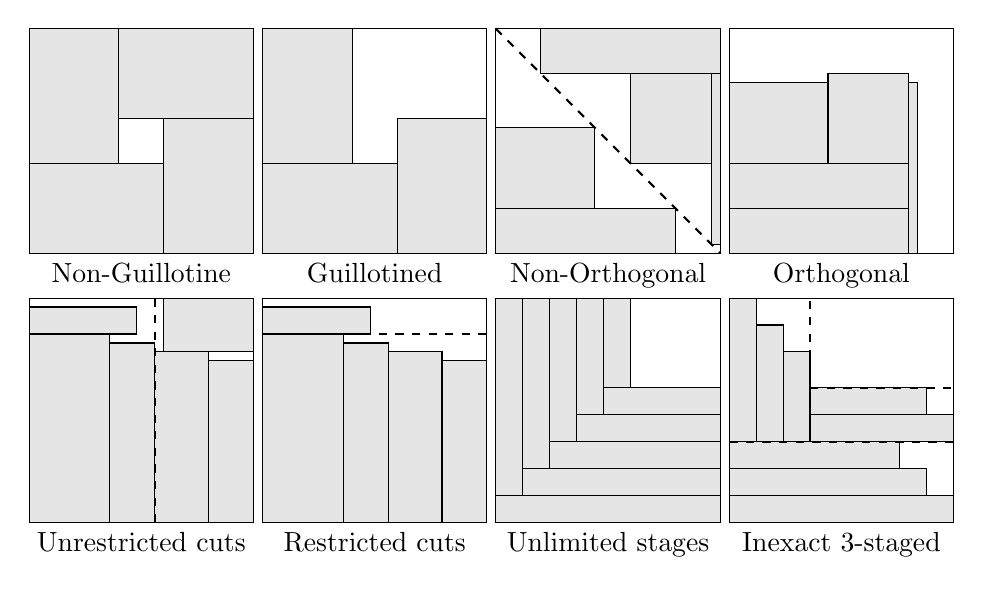
\begin{tikzpicture}[scale=0.114]
\def\piececolor{gray!20}
\def\labelxshift{12.5}
\def\labelyshift{0}
\def\labelfontsize{\normalsize}
\begin{scope}[shift={(0, 0)}] % FIRST ROW
\begin{scope}[shift={(0, 0)}] % FIRST IMAGE
\draw (0,0) rectangle +(25, 25);
\draw[fill=\piececolor] (0, 0) rectangle +(15, 10);
\draw[fill=\piececolor] (15, 0) rectangle +(10, 15);
\draw[fill=\piececolor] (0, 10) rectangle +(10, 15);
\draw[fill=\piececolor] (10, 15) rectangle +(15, 10);

\node [below] at (\labelxshift, \labelyshift) {\labelfontsize Non-Guillotine};
\end{scope}

\begin{scope}[shift={(26, 0)}] % SECOND IMAGE
\draw (0,0) rectangle +(25, 25);
\draw[fill=\piececolor] (0, 0) rectangle +(15, 10);
\draw[fill=\piececolor] (15, 0) rectangle +(10, 15);
\draw[fill=\piececolor] (0, 10) rectangle +(10, 15);
%\draw[fill=\piececolor] (10, 10) rectangle +(15, 10);

\node [below] at (\labelxshift, \labelyshift) {\labelfontsize Guillotined};
\end{scope}

\begin{scope}[shift={(52, 0)}] % THIRD IMAGE
\draw (0,0) rectangle +(25, 25);
\draw[fill=\piececolor] (0,0) rectangle +(20, 5);
\draw[fill=\piececolor] (0,5) rectangle +(11, 9);
\draw[fill=\piececolor] (5, 20) rectangle +(20, 5);
\draw[fill=\piececolor] (15, 10) rectangle +(9, 10);
\draw[fill=\piececolor] (24, 1) rectangle +(1, 19);

\draw[dashed, thick, black] (0, 25) -- (25, 0);]

\node [below] at (\labelxshift, \labelyshift) {\labelfontsize Non-Orthogonal};
\end{scope}

\begin{scope}[shift={(78, 0)}] % FOURTH IMAGE
\draw (0,0) rectangle +(25, 25);
\draw[fill=\piececolor] (0,0) rectangle +(20, 5);
\draw[fill=\piececolor] (0, 10) rectangle +(11, 9);
\draw[fill=\piececolor] (0, 5) rectangle +(20, 5);
\draw[fill=\piececolor] (11, 10) rectangle +(9, 10);
\draw[fill=\piececolor] (20, 0) rectangle +(1, 19);

\node [below] at (\labelxshift, \labelyshift) {\labelfontsize Orthogonal};
\end{scope}
\end{scope}

\begin{scope}[shift={(0, -30)}] % SECOND2 ROW
\begin{scope}[shift={(0, 0)}] % FIRST IMAGE
\draw (0,0) rectangle +(25, 25);

%\draw[fill=\piececolor] (0,0) rectangle +(6, 19);
%\draw[fill=\piececolor] (6,0) rectangle +(5, 18);
\draw[fill=\piececolor] (14,0) rectangle +(6, 19);
\draw[fill=\piececolor] (20,0) rectangle +(5, 18);
\draw[fill=\piececolor] (0,0) rectangle +(9, 21);
\draw[fill=\piececolor] (9,0) rectangle +(5, 20);
%\draw[fill=\piececolor] (0,19) rectangle +(10, 6);
\draw[fill=\piececolor] (15,19) rectangle +(10, 6);
\draw[fill=\piececolor] (0,21) rectangle +(12, 3);

\draw[dashed, thick, black] (14, 0) -- (14, 25);

\node [below] at (\labelxshift, \labelyshift) {\labelfontsize Unrestricted cuts};
\end{scope}

\begin{scope}[shift={(26, 0)}] % SECOND IMAGE
\draw (0,0) rectangle +(25, 25);

%\draw[fill=\piececolor] (0,0) rectangle +(6, 19);
%\draw[fill=\piececolor] (6,0) rectangle +(5, 18);
\draw[fill=\piececolor] (14,0) rectangle +(6, 19);
\draw[fill=\piececolor] (20,0) rectangle +(5, 18);
\draw[fill=\piececolor] (0,0) rectangle +(9, 21);
\draw[fill=\piececolor] (9,0) rectangle +(5, 20);
%\draw[fill=\piececolor] (0,19) rectangle +(10, 6);
%\draw[fill=\piececolor] (15,19) rectangle +(10, 6);
\draw[fill=\piececolor] (0,21) rectangle +(12, 3);

\draw[dashed, thick, black] (0, 21) -- (25, 21);

\node [below] at (\labelxshift, \labelyshift) {\labelfontsize Restricted cuts};
\end{scope}

\begin{scope}[shift={(52, 0)}] % THIRD IMAGE
\draw (0,0) rectangle +(25, 25);

\draw[fill=\piececolor] (0,0) rectangle +(25, 3);
\draw[fill=\piececolor] (0,3) rectangle +(3, 22);
\draw[fill=\piececolor] (3,3) rectangle +(22, 3);
\draw[fill=\piececolor] (3,6) rectangle +(3, 19);
\draw[fill=\piececolor] (6,6) rectangle +(19, 3);
\draw[fill=\piececolor] (6,9) rectangle +(3, 16);
\draw[fill=\piececolor] (9,9) rectangle +(16, 3);
\draw[fill=\piececolor] (9,12) rectangle +(3, 13);
\draw[fill=\piececolor] (12,12) rectangle +(13, 3);
\draw[fill=\piececolor] (12,15) rectangle +(3, 10);

\node [below] at (\labelxshift, \labelyshift) {\labelfontsize Unlimited stages};
\end{scope}

\begin{scope}[shift={(78, 0)}] % FOURTH IMAGE
\draw (0,0) rectangle +(25, 25);
\draw[fill=\piececolor] (0,0) rectangle +(25, 3);
%\draw[fill=\piececolor] (0,3) rectangle +(3, 22);
\draw[fill=\piececolor] (0,3) rectangle +(22, 3);
%\draw[fill=\piececolor] (3,6) rectangle +(3, 19);
\draw[fill=\piececolor] (0,6) rectangle +(19, 3);

\draw[fill=\piececolor] (0,9) rectangle +(3, 16);
\draw[fill=\piececolor] (9,9) rectangle +(16, 3);
\draw[fill=\piececolor] (3,9) rectangle +(3, 13);
\draw[fill=\piececolor] (9,12) rectangle +(13, 3);
\draw[fill=\piececolor] (6,9) rectangle +(3, 10);

\draw[dashed, thick, black] (0, 9) -- (25, 9);
\draw[dashed, thick, black] (9, 9) -- (9, 25);
\draw[dashed, thick, black] (9, 15) -- (25, 15);

\node [below] at (\labelxshift, \labelyshift) {\labelfontsize Inexact 3-staged};
\end{scope}
\end{scope}
\end{tikzpicture}

\caption{Examples of valid patterns for most of the discussed problem variants. In \emph{Non-Orthogonal}, \emph{Unrestricted cuts}, and \emph{Restricted cuts}, the dashed line indicate the first cut of the pattern. In \emph{Inexact 3-staged}, the dashed line separates the three stages.}
\label{fig:qualifier_examples}
\end{figure}

The Remark~1 and Example~1 were imprecise and were thoroughly rewritten. A new diagram was added close to them to help understanding Example~1. The changes follow:

\begin{remark}
\oldtext{If a normal cut~\(q\) divides the size-normalized plate~\(j\), the first child is always size normalized, but the second child may not be size normalized.}
\newtext{If a normal cut divides a size-normalized plate, then the dimension perpendicular to the cut, in the first child, is normalized. The dimension parallel to the cut in the first child, and both dimensions of the second child, are not guaranteed to be normalized.}
\end{remark}

\begin{example}\label{ex:renormalization_after_cut}
\oldtext{Given two pieces with \(l = [5, 7]\), \(u = [2, 3]\), and a size-normalized plate of length~\(21\), a normal cut at~\(12\) creates a non-normalized second child of length~ \(9\).}
\newtext{Consider three pieces with~\(l = [5, 7, 9]\), \(w = [6, 4, 11]\), \(u = [3, 1, 1]\), and a plate of dimensions \(15\)x\(15\). The plate dimensions are already normalized. The plate length matches stacking the three copies of the first piece. The plate width matches laying side-by-side the other two pieces. An horizontal cut at length~\(7\) is a normal cut because it matches the length of the second piece. If the cut is done, the width of both children is not normalized anymore, nor is the length of the second child. The width of both children is not normalized because the third piece does not fit either child so, for both children, the largest width a valid packing may reach is~\(12\). The length of the second child is not normalized because the largest length a valid packing inside the second child may reach is 7. The dimensions of both children may be normalized to \(7\)x\(12\). This example already shows an immediate gain, instead of creating two new plate sizes, the enumeration only creates a single new plate type. The cut creates two copies of this single type of plate.}
\end{example}

\begin{figure}[ht]
\center
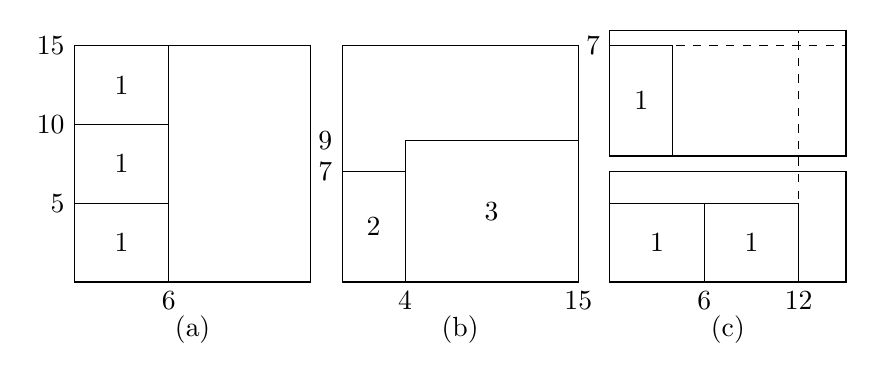
\begin{tikzpicture}[scale=0.20]
\begin{scope}[shift={(0, 0)}]
\draw [draw=black]   (0, 0) rectangle ++(15, 15);
\draw [draw=black]   (0, 0) rectangle     ++(6, 5) node [midway] {1};
\draw [draw=black]   (0, 5) rectangle     ++(6, 5) node [midway] {1};
\draw [draw=black] (0, 10) rectangle     ++(6, 5) node [midway] {1};
\node [left]  at (0, 5) {5};
\node [left]  at (0, 10) {10};
\node [left]  at (0, 15) {15};
\node [below]  at (6, 0) {6};
\node [below] at (7.5, -1.5) {(a)};
\end{scope}
\begin{scope}[shift={(17, 0)}]
\draw [draw=black]   (0, 0) rectangle ++(15, 15);
\draw [draw=black]   (0, 0) rectangle     ++(4, 7) node [midway] {2};
\draw [draw=black]   (4, 0) rectangle   ++(11, 9) node [midway] {3};
\node [below]  at   (4, 0)   {4};
\node [below]  at (15, 0) {15};
\node     [left]  at   (0, 7)   {7};
\node   [left]  at (0, 9)   {9};
\node [below] at (7.5, -1.5) {(b)};
\end{scope}
\begin{scope}[shift={(34, 0)}]
\draw [draw=black]   (0, 0) rectangle ++(15, 7);
\draw [draw=black]   (0, 0) rectangle     ++(6, 5) node [midway] {1};
\draw [draw=black]   (6, 0) rectangle     ++(6, 5) node [midway] {1};
\node [below]  at (6, 0) {6};
\node [below]  at (12, 0) {12};
\draw[dashed] (12, 0) -- (12, 16);

\draw [draw=black]   (0, 8) rectangle ++(15, 8);
\draw [draw=black]   (0, 8) rectangle   ++(4, 7) node [midway] {1};

\node     [left]  at   (0, 15)   {7};
\draw [dashed] (0, 15) -- (15, 15);
\node [below] at (7.5, -1.5) {(c)};
\end{scope}
\end{tikzpicture}
\caption{\newtext{Diagram of~\autoref{ex:renormalization_after_cut}: (a) the three copies of the first piece stacked; (b) the second and third pieces side-by-side; (c) both children of an horizontal normal cut over a normalized plate are not normalized themselves.}}
\end{figure}
TODO: We have diagrams for every characteristic of the problem (we used those in the proposal presentation), however, we will probably merge all of them in a super-diagram or it will take too much space. Example 1 probably can use a diagram, but it needs to be fixed first. The remark 1, in which the example is based, is wrong. I need to fix it first (there is a corner case I did not thought before submitting the paper).
\end{answer}

\begin{concern}
No justification or explanation for the datasets is provided, besides citations. Apart from their difficulty, why are these interesting problems? Are they synthetic? Do they come from industry applications?
\end{concern}
\begin{answer}\label{ans:dataset_info}
We added a some extra context close to the first mention of every dataset. For the 59 instances dataset from~\cite{furini:2016}:

\newtext{The chosen dataset is, therefore, the same as the one used in these works for the comparison to be possible. The dataset aggregates 59 instances of the previous literature from many distinct sources, all instances are either artificially generated, or of indisclosed origin.}

For the 80 instances dataset from~\cite{velasco:2019}:

\newtext{The instances were artifically generated and are divided in four classes of 20 instances each. The dataset focus on two characteristics: (i) the area of the pieces is small compared to the area of the original plate (the average ratio vary between 1.6\% and 5\%); (ii) each class is defined by the shape of the original plate, and the likely shape of the randomly generated pieces. The original plates of the first two classes have one dimension two or four times larger than the other dimension. In the first class, the pieces are likely to be larger in the same dimension the original plate is larger; while, in the second class, the pieces are likely to be larger in the dimension the original plate is shorter. The original plates of the last two classes are squares. The pieces of the third class have, in average, the same dimension with double the size of the other; while, in the fourth class, half of the pieces follow the previous distribution, and the other half invert the favored dimension.}

We have also added the following sentence to the caption of current Table 5 (previously Table 6): \newtext{The instance names follow the pattern \texttt{Class\_L\_W\_n\_seed}.}
\end{answer}

\begin{concern}
I don't view Section 5.2 on the choice of LP algorithm as essential to the main point of the paper. It could be replaced with a few sentences saying that you use the barrier method for the root node and dual simplex otherwise, based on experiments you performed.\label{con:remove_sec_5_2}
\end{concern}
\begin{answer}
The entire former Section 5.2 (`The choice of LP algorithm') was replaced by following sentences:
\newtext{For the root node relaxation of the final built model, the barrier algorithm was employed (\texttt{Method}~\(= 2\)). Whenever the run included the pricing phase, the multiple continuous relaxations from such phase were solved by the dual simplex algorithm~\texttt{Method}~\(= 1\). In preliminary experiments, barrier took less time than dual simplex to solve a model relaxation from scratch. However, if a previous base can be exploited, as it is the case during the pricing phase, choosing dual simplex over barrier made the pricing phase take less time.}
\end{answer}

\begin{concern}
This is more of a style issue, but I find the tables very hard to read. The abbreviations are entirely nonstandard. If using non-standard abbreviations, please define them in the table caption so that it's possible to interpret the table without having to scan through the main text to find the definitions of the labels.
\end{concern}
\begin{answer}
We have moved the paragraphs explaining the columns of each table to the caption of the corresponding table. These changes are not marked in color in the text, as the changes to the text (besides making them a part of the caption) are minimal.
\end{answer}

\begin{concern}
Table 5 presents instances by `instances classes' numbered from 1 to 4. No explanation of these classes is provided, besides a reference to [29]. Information like this that's essential to interpreting the results should be included in the paper.
\end{concern}
\begin{answer}
This concern ended up being addressed in~\autoref{ans:dataset_info}.
\end{answer}

\begin{concern}
I don't understand the statement in the conclusion about the `almost serial root node relaxation phase'. Gurobi's barrier method can run multi-threaded in the same way that branch-and-bound does (\url{https://support.gurobi.com/hc/en-us/articles/360013419951-Does-using-more-threads-make-Gurobi-faster-}). Why is it `almost serial'? Are you referring to a crossover step?
\end{concern}
\begin{answer}
The statement was reworked, but first we explain our previous statement. The Gurobi's barrier method was run multithreaded but it had some drawbacks: (i) for deterministic runs, as it is our case, Gurobi reports a `Concurrent spin time' which indicates the time lost by the threads because they are blocked by other threads; (ii) nor the initial ordering, nor the crossover step seem to benefit from multiple threads. TODO: rework section to mention: (i) why we believe the root node relaxation benefits less from multithreading; (ii) that only barrier benefits, what can be unfair to some formulations; (iii) and how the increase of time in the root node relaxation affects other points (risk of ending without primal solution, and there is not time to explore many nodes, so the B\&B parallelisation is also less effective, citing the same Gurobi url).
\end{answer}

\begin{concern}
References 7 and 8 are identical.\\Page 5 typo: `et all' should be `et al.'\\Page 5 typo: `MiM main gain' should be `MiM's main gain'\\Page 7 typo: `\(y_j, i \in \bar{J}\)' should be `\(y_j, j \in \bar{J}\)'
\end{concern}
\begin{answer}
The problem with the identical references is fixed. There is no \emph{et all} in page 5, instead there is an use of \emph{et alii}, which is the correct Latin form for masculine plural and, therefore, the correct form in that context. Also in page 5, `MiM main gain' was used instead of `MiM's main gain' because we follow a style guide that discourages the apostrophe to denote the possessive of inanimate objects. The whole paper follows this guideline. In this case, we decided to change the text to `The main gain of MiM [...]'. The typo in page 7 was fixed, the correct notation is~\(y_i, i \in \bar{J}\) (i.e., the index should have been \(i\)). This last change was also impacted by~\autoref{con:sec3_concerns} which asks for a more consistent usage of indices.
\end{answer}

\begin{concern}
The code has very minimal testing (see \url{https://github.com/henriquebecker91/GuillotineModels.jl/blob/0.2.2/test/run_model_solving_tests.jl}). Given the impenetrability of the code and the lack of tests, it's hard for me to say much about the correctness of the results.\label{con:minimal_testing}
\end{concern}
\begin{answer}
The test suite of a julia package is intended automatically on continuous integration servers and, to avoid timeouts, is limited to checking the basics. The current version of the package (0.8.7) has a slightly improved test suite (it also checks the reading of all the supported instance formats) and it is passing all current tests. Most of the evidence of the correctness of the results comes not from the package test suite, but instead from: (1) the check of the optimal solution value of the older dataset of 59 instances, which was done in \url{https://github.com/henriquebecker91/phd/blob/master/latex/revised_PPG2KP/notebooks/Comparison_analysis.jl#L91--L107} (in fact, we found that \cite{furini:2016} incorrectly reports an optimal value of 22503 for okp2, the correct value is 22502 which is also obtained by~\cite{fekete:1997}); (2) the fact there is no inconsistency between the lower and upper bounds we found in our last table and the ones found by~\cite{velasco:2019}; (3) for the base formulation from~\cite{furini:2016} we obtain the number of variables down to the exact number; (4) the mathematical proof of correctness presented in the paper. Unit tests are not so useful because the most natural way to validate any reduction is either by mathematical proof (as presented in this paper) or by obtaining optimal results for a large amount of instances (integration testing, also done in the paper). There is little guarantee an unit test will catch a corner case that does not appear in any literature instance.
\end{answer}

\begin{concern}
As it relates to the usefulness of the code for the community, the public readme at \url{https://github.com/henriquebecker91/GuillotineModels.jl} has no information on how to use the code.\label{con:no_readme}
\end{concern}
\begin{answer}
The code documentation is now available at~\url{https://henriquebecker91.github.io/GuillotineModels.jl/stable/} which is linked in the mentioned public README~(\url{https://github.com/henriquebecker91/GuillotineModels.jl}). The README now explains: how to install Julia; how to install the \inlinecode{GuillotineModels.jl} package; where is located a script that may be used to solve instances without needing to program in Julia; how to use call said script; how to read the output of the script; which input formats are accepted; and gives the script list of parameters, and their explanation, which is also available by calling the script and passing the parameter \inlinecode{--help}.
\end{answer}

\begin{concern}
There is function-level documentation in comments and at \inlinecode{\mytilde/.julia/packages/GuillotineModels/dIWFD/docs/build/index.html}, but I don't find it close to sufficient for figuring out how to use the code. There are no tutorials, how-to guides, or explanations of concepts.\label{con:no_tutorial}
\end{concern}
\begin{answer}
The code documentation (available at~\url{https://henriquebecker91.github.io/GuillotineModels.jl/stable/}) has now an explanation of the utility of each module, and points out four new code examples that come with the package installation. These should be able to help a new user to understand how to accomplish some simple tasks with the help of the package.
\end{answer}

\begin{concern}
I tried to understand what should be a relatively simple part of the code, \inlinecode{get\_cut\_pattern()} in \inlinecode{get\_cut\_pattern.jl}, which reconstructs the sequence of cuts given a solution to the MIP. \inlinecode{get\_cut\_pattern()} calls \inlinecode{\_get\_cut\_pattern()}, where the real work is done. \_\inlinecode{get\_cut\_pattern()} has arguments named \inlinecode{nzpe\_idxs}, \inlinecode{nzpe\_vals}, \inlinecode{nzcm\_idxs}, and \inlinecode{nzcm\_vals}. These arguments are untyped, and without a forensic analysis it's hard for me to figure out their structure and what assumptions are made on the input. Another argument to \inlinecode{\_get\_cut\_pattern()} is of type \inlinecode{ByproductPPG2KP}. The definition of this type is heavily templated (making it hard to follow) and I didn't find the fields sufficiently documented to understand how they're used in \inlinecode{\_get\_cut\_pattern()}.\label{con:get_cut_pattern_not_understood}
\end{concern}
\begin{answer}
The \inlinecode{get\_cut\_pattern} is probably the most complex function (in terms of human comprehension, not computational effort) of the package.
The method should be able to recover solutions from both the Furini's formulation as well as our formulation, independently of which reductions were applied.
The way both formulations works also makes this process to be not straightforward.
The value of the variables inside a model represent a class of possible solutions not a single concrete solution.
When multiple plates of the same dimensions are present, there is no information from exactly which larger plate they were cut from (this is intended, as this is a source of symmetries in the model).
The procedure must, therefore, concretize one of the multiple symmetric solutions possible.
More than this, the function now also support the variants of the formulation that solve the Cutting Stock Problem and the Multiple Knapsack Problem (both of which have multiple original plates, not just one).
The function in question starts with a 17-line comment explaining how it works, and then have more comments further. \emph{We have further improved its comments}\footnote{See: \url{https://github.com/henriquebecker91/GuillotineModels.jl/commit/c68c07653e57f190e0b3e392ff75b60897912897}}, but we found necessary to point out that it is a complex procedure at its core, and making it trivial to follow is not a reasonable goal.
Finally, about the lack of types for some parameters (e.g., \inlinecode{nzpe\_idxs}, \inlinecode{nzpe\_vals}, \inlinecode{nzcm\_idxs}, and \inlinecode{nzcm\_vals}), this is a Julia language guideline\footnote{See: \url{https://docs.julialang.org/en/v1/manual/style-guide/\#Avoid-writing-overly-specific-types}}. The basic idea is that parameters should be documented, but their allowed types should not be restricted without need. We had, in fact, not documented these parameters, as they belong to an internal function; but this was rectified in the same commit as the comments improvements we mentioned above.
\end{answer}

\begin{concern}
The \inlinecode{extract\_data.jl} script mentions a `\inlinecode{finished\_experiments}' folder. This isn't present, from what I can tell. It would be useful to have these for the purpose of validating the results processing pipeline, especially given that \inlinecode{run\_experiments.jl} has a `good chance it will stop with error, because some few runs take more than 32 GiB of RAM'.
\end{concern}
\begin{answer}
We apologize for this oversight. The code was downloaded by means of the git repository. We do not save the raw data in the git repository because of the sheer volume of it. The raw data yet exists and we have uploaded it to the following link: \url{https://drive.google.com/file/d/1H7zKXKyTG9tXaxWwTlx_G80nCyGc6SR4/view?usp=sharing}
\end{answer}

\begin{concern}
It's common to see commented-out and unused code, like \inlinecode{run\_experiments} in \inlinecode{run\_experiment.jl}, and the file \inlinecode{abandoned.jl}. These are distracting for anyone reading the code and should be removed.\label{con:abandoned_code}
\end{concern}
\begin{answer}
The file \inlinecode{abandoned.jl} and some comments in the \inlinecode{GuillotineModels.jl} repository were removed. These changes can be seen in the following commit: \url{https://github.com/henriquebecker91/GuillotineModels.jl/commit/698bbad8c2f0a1538cd58b9e07e916a00d979d88}. We decided to preserve the comments in~\inlinecode{run\_experiment.jl} for historical reasons.
\end{answer}

\section{Anonymous Referee \#2}

\textbf{General commentary:} ``{\itshape
The paper does not present a new theoretical deep contribution nor a completely new methodology to tackle the G2KP. However as explained above, the paper presents two methodological improvements for the state-of-the-art MILP G2KP formulation. These two ideas allows to improve the performance of GUROBI used to solve the obtained smaller models. The paper for sure has merit, and I would probably suggest a mayor revision in several OR journals, like e.g., European Journal of Operational Research or Computers \& Operations Research. However, I am not sure that the contribution is enough to meet the very hight standards of Mathematical Programming Computation, one of the flagship journals of the domain.
}''

\bigskip

\begin{concern}
One of the more interesting computational results of the paper in my opinion is that with the new `reduction' techniques it is not necessary anymore to price out the variables of the MILP formulation. From the computational results, it clearly emerges that even if the size of the model can be reduced no computational benefits can be achieved. This is clearly not the case for the original MILP formulation where the pricing of the variables is a crucial step. I think that it would be interesting to further dig this important point since apparently the new formulation is small enough and no additional reduction based on the pricing of the variables are necessary. It seems to be the case also for the larger instances of the second testbed. Is it linked to the powerful preprocessing techniques employed by GUROBI? Is it possible to explain this important fact also from a theoretical point of view? Is it a sort of reduced-cost fixing?
\end{concern}
\begin{answer}
TODO: when we describe the pricing procedure better this will allow us to better explain (or at least, hypothetize) why any further reductions done by the pricing do not generally improve the performance.
\end{answer}

\begin{concern}
Abstract: please rewrite the first two lines using the names of the procedure proposed in the paper. In addition, since you only tests the knapsack problem please update the title accordingly. I agree that the techniques proposed are (quite) general and can be applied also to other families of guillotine 2D Cutting problems, but in this paper the authors only address the knapsack problem so I found the title slightly misleading. Please remove the specific percentages of variables and constraints, i.e., 3.07\% and 8.35\%. You have several models and it is not clear to which variant they refer (also these number are not commented in the computational section if I’m not mistaken). I would also reduce the list of computational results of the paper in the abstract to shorten it a bit.
\end{concern}
\begin{answer}
The title was changed in the following way: Enhanced Formulation for \newtext{the} Guillotine 2D Cutting \newtext{Knapsack} Problem\oldtext{s}

The abstract was modified in the following fashion:

We advance the state of the art in Mixed-Integer Linear Programming (MILP) formulations for Guillotine 2D Cutting Problems by (i) adapting a previously-known reduction to our preprocessing phase \newtext{(plate-size normalization)} and by (ii) enhancing a previous formulation \newtext{(PP-G2KP from Furini et alli)} by cutting down its size and symmetries.
Our focus is the Guillotine 2D Knapsack Problem with orthogonal and unrestricted cuts, constrained demand, unlimited stages, and no rotation -- however, the formulation may be adapted to many related problems.
The code is available.
\oldtext{Concerning the set of 59 instances used to benchmark the original formulation, and summing the statistics for all models generated, the enhanced formulation has only a small fraction of the variables and constraints of the original model (respectively, 3.07\% and 8.35\%).}
\newtext{Concerning the set of 59 instances used to benchmark the original formulation,} the enhanced formulation \oldtext{also} takes about 4 hours to solve all instances while the original formulation takes 12 hours to solve 53 of them (the other six runs hit a three-hour time limit each).
We integrate, to both formulations, a pricing framework proposed for the original formulation; the enhanced formulation keeps a significant advantage in this situation.
Finally, in a recently proposed set of 80 harder instances, the enhanced formulation (with and without the pricing framework) found: 22 optimal solutions \oldtext{for the unrestricted problem} (5 already known, 17 new); \oldtext{22 optimal solutions for the restricted problem (all are new and they are not the same 22 of the optimal unrestricted solutions);} better lower bounds for 25 instances; better upper bounds for 58 instances.

\end{answer}

\begin{concern}
Section 1: `If we further qualify the G2KP, we only mean to discard the qualifiers above that directly conflict with the extra qualifiers, if any.' This second sentence of the paper is not understandable by the reader at this very point. Please remove it or put it after the description of the variants of the G2KP.
\end{concern}
\begin{answer}
The sentence now takes place after the description of the variants of the G2KP. We also added the following sentence after it:
\newtext{For example, if we refer to the \emph{unconstrained G2KP}, then we meant to discard the constrained qualifier but keep the remaining qualifiers, i.e., no rotation, unlimited stages, as well as guillotined, orthogonal, and unrestricted cuts.}
\end{answer}

\begin{concern}
`A consequence of this rule is that we often do not obtain the pieces directly from the original plate', all the pieces are obtained by the original plate, please rephrase it or better explain.
\end{concern}
\begin{answer}
We decided to remove the sentence because it was not essential and only led to confusion. The sentence was targeted to readers that were not familiar with the guillotine constraint. The purpose was to show that intermediary plates are an immediate consequence of this constraint. We now believe even a novice will be able to perceive this connection without the help of this sentence.
\end{answer}

\begin{concern}
In the paragraph which starts with `Constrained demand means [...]', the description is not clear since, clearly, an upper bound on the number of copies \(u_j\) can be always set. First of all I think you wanted to say `strongly' NP-Hard (the problem clearly remains difficult also with unconstrained demands). For instance, just considering the area bound, \(u_j \leq \lfloor \frac{L \cdot W}{l_j \cdot w_j} \rfloor\). Is this bound better that the one you present, i.e.,\(u_j < \lceil L / l_j \rceil \cdot \lceil W / w_j \rceil\) (by the way, where does this bound come from?). Consider for instance \(L = W = 10\) and one piece~\(j\) with \(l_j = 9\) and \(w_j = 1\), the two upper bounds are different I think, and probably even stronger bounds can be computed.\label{con:constrained_NP_hard_first}
\end{concern}
\begin{answer}
Your guess is correct: we intended to say \emph{strongly} NP-hard. We apologize for the flagrant error. This error is now fixed. The bound had a typo, we intended to say~\(u_j < \lfloor L / l_j \rfloor \cdot \lfloor W / w_j \rfloor\), i.e., the instead of the round up we intended to round down. However, this trivial bound is only valid for no-rotation variants and it may cause some confusion at this point of the text. In the end, we have reworked the text to make more explicit the importance of the demand bounds for the constrained/unconstrained variants and suppressed an explicit bound, the new text follows:
\newtext{Consequently, if~\(u_i \geq \beta_i : \forall i \in \bar{J}\), where \(\beta_i\) is an upper bound on the number of copies of piece~\(i\) that can be produced from the original plate, then the instance is probably better solved as an instance of the unconstrained G2KP instead. We avoid this kind of instances in our experiments.}
\end{answer}

\begin{concern}
Finally, you mention the minimization of the waste but then you do not use it. As a general rule, please introduce and explain only the things you use in the paper.
\end{concern}
\begin{answer}
TODO: here we can suppress the mention to waste minimization, or we can point out which datasets have weighted and unweighted instances in our datasets.
\end{answer}

\begin{concern}
Finally, a picture would also be important to understand the different variants of the G2KP, in my opinion.
\end{concern}
\begin{answer}
The same was suggested in~\autoref{con:diagrams_for_problem} and this suggestion is addressed there.
\end{answer}

\begin{concern}
Motivation: `A better MILP [...]' please say in terms of what. `a better continuous relaxation [...]', the model provided has the same LP relaxation value of the original model, right? This point is not discussed in the paper and I think it is important to mention it. Instead, this entire paragraph on the motivation is quite straightforward. I think that you can reduce the entire paragraph to one sentence, the reader of MPC knows all the benefits of advanced MILP techniques. Finally, what do you mean by `anytime procedures'?
\end{concern}
\begin{answer}
TODO: we need to check if we will present LP relaxations, because in the paper with Martin we have seen a slightly improve in the relaxations compared to the the Furini's model. ALREADY WRITTEN: The expression `anytime procedures' refer to optimization methods that give a solution of adequate quality when stopped at any timeframe, for example: starting with fast heuristics to have a solution of good quality if the method is stopped within a single second, and then switching to methods that take more time to deliver good results but are able to reach near-optimal solutions given enough time. An example of thesis focused on the subject is available at \url{https://d-nb.info/1018257942/34}. We believed `anytime procedures' was a widely known concept but further investigation has shown us that the jargon is not as widespread as we thought.
\end{answer}

\begin{concern}
Related works: `points out three strategies employed by previous exact solving methods which cause loss of optimality' are you speaking of exact methods, right? Are you saying that there are mistakes in these papers? It is not clear, what do you mean by `which cause loss of optimality'?
\end{concern}
\begin{answer}
Yes, the survey points out there are mistakes in these papers. The sentence was changed to make it more clear: `Moreover, \cite{russo:2020}~points out three strategies employed by previous exact solving methods which cause loss of optimality\newtext{, i.e., these methods cannot be considered exact anymore}.'
\end{answer}

\begin{concern}
Related works: [...] You say `Consequently, while it may be interesting for completeness sake, we do not compare against the formulations proposed in [19, 21, 22].' I am fully aware that comparing results on different machines is difficult and cannot be extremely precise. However, many papers do it by simply comparing the order of magnitude of the numbers presented in the tables (or scaling according to the available benchmarks). I think that you can do something similar to compare your approach to these approaches as well. It would add for sure value to the paper.
\end{concern}
\begin{answer}
Unfortunately, since we have sent this paper for evaluation in MPC, we and the authors of the mentioned papers have partnered to write a conference paper that is already under evaluation. Considering that one of the main contributions of this new paper is a comprehensive comparison of these methods, we prefer to keep the lack of comparison, instead of risking the addition of content under evaluation elsewhere.
\end{answer}

\begin{concern}
Section 3: I understand the procedure called `(i) (ii) (iii) (iv)', but I think that an example would help the reader to better understand. You also have to formally define the set of all residual panels which are obtained thanks to the cuts. What is \(j\) in formula (1) ? Before \(j\) has been used to define an item, here it should be a plate, but the set of all plates is not defined. In addition proposition (1) works with other plates, i.e., the index \(k\). It is necessary to define the range of the indices used. Summarizing, I think it is necessary to define the entire procedure you used to create the set of all residual panels starting from the normal cuts. Please add an sentence explaining the main idea behind proposition (1) and give a numerical example. Checking this condition increases the computational complexity of the enumeration of the panels? Example 1, is not clear, I would encourage the authors to add several complete examples to explains the main steps. They help a lot in understanding.\label{con:sec3_concerns}
\end{concern}
\begin{answer}
About Example 1, \autoref{con:ex1_and_more_diagram} also asked for its improvement and we addressed it there.
TODO: go back from introduction and change every index in \(\bar{J}\) (the piece set) to \(i\) and keep \(j\) and \(k\) for plates that may or may not be piece-sized (i.e., elements of \(J\)). This should help the text to be more clear.
TODO: Give an example for `(i) (ii) (iii) (iv)' (it may be a little hard to find a good real example, but if found it will take only a paragraph). The paragraph just before formula (1) defines~\(j\) can be any plate, \(N_{jo}\) gives the normal cuts of orientation \(o\) for plate \(j\), the set of all plates does not need to be defined for this definition to work (only its dimensions need to be known and the set of pieces). Check where \(j\) is used as a piece. Be more clear that \(k\) also works over plates? (Not sure what is the source of confusion here. The entire procedure is kinda out of the scope of this work, as we would need to re-explain two reductions from Furini. Add the sentence about preposition 1 (a low-level one, I think it is what it is asking) and a numerical example. The complexity is not increased because every normal size was already computed, and in \(O(W + L)\) it is possible to create two vectors that allow \(O(1)\) mapping between a width/length to the corresponding normalized width/length. Improve example 1.
\end{answer}

\begin{concern}
Section 4.1: as you correctly say, the number of variables can also increase, can you clearly states which are the conditions under which the total number decreases. Please formalize the theorem using a mathematical notation. It is clear what you mean but it is not precise enough in my opinion. The same applies to the proof, which seems to be correct (the theorem is quite intuitive), but it lacks of formalization. In addition, I think that a couple of figures would help a lot to understand the difference cases.
\end{concern}
\begin{answer}
We do believe the referee meant Section 4.2 (The revised variable enumeration). TODO: about the number of variables, the number decreases if the amount of cuts after the plate midpoint is larger than the number of extraction variables added. There is no closed formula for it and the two ways of computing the variables need to be done and compared. Check on how to formalize more the proof and add images (this was also asked by Ritt).
\end{answer}

\begin{concern}
[...] my first general consideration is to remove or at least limit the flow of the presentation on the computational `fight' between the formulations called \emph{faithful} (the re-implementation of the MILP model of the IJOC paper) and \emph{enhanced} (the new one). Apart from the presence of the extraction variables, these two formulation are exactly the same, they both are pseudo-polynomial size MILP formulations whose size depend on the number of number of residual plates (i.e., the cutting position). What I’m trying to say is that once demonstrated that \emph{enhanced} is smaller than \emph{faithful} in terms of number of variables and constraints then it is not necessary to tests \emph{faithful} anymore. For instance, it is not necessary to tests all the techniques on both formulation as done in table 3. It is hard to follow and unnecessary in my opinion.
\end{concern}
\begin{answer}
The number of variables and constraints in a model is not a good indicator of its performance, \emph{even if both models come from the same formulation}.
The \emph{purge} procedure we mentioned in the pre-review manuscript was able to reduce the number of variables and constraints by~60\mytilde70\% after the pricing procedure, and this reduction was shown to have basically no effect over the solver performance.
The solver itself was already able to disregard most of these variables and constraints.
The same way, our enhanced formulation could be only removing variables and constraints that were recognized as unnecessary by the solver, and which had no impact over the solver run time.
We believe it is necessary to keep the comparison to guarantee to the reader the enhanced formulation does not only impact proxy measurements like model size, but actually make it easier for the solver to solve the model.
Another question a reader could postulate is: if enhancements like the plate-size normalization, which is compatible with both original and enhanced formulations, could close the gap between the formulations.
This is, if when applied to the original model, this technique would also remove the variables abstracted away by the enhanced formulation.
In such a case, the enhanced formulation would have far less value, as it would be simpler to keep the original formulation with an extra preprocessing step, instead of changing both formulation and preprocessing.
For this reason we also do not suppress the application of different techniques to the original formulation.
\end{answer}

\begin{concern}
please concentrate only on the important points. I do not think that section 5.2 is necessary and important. One sentence is enough, simply saying that the barrier is fast when no reoptimization is necessary. It is a well known fact in the community. You can say in one sentence when you use the dual simplex and when the barrier algorithms. No other details are necessary in my opinion (maybe in the appendix). Instead, it is important to describe at least the main ideas of the pricing procedure and how it is executed.\label{con:describe_pricing}
\end{concern}
\begin{answer}
About removing Section 5.2, the same was suggested in~\autoref{con:remove_sec_5_2} and it is addressed there (the section was replaced by a short paragraph).
The lack of a condensed explanation of the pricing procedure was also noted in~\autoref{con:describe_pricing_2}. \autoref{con:not_self_contained} asks for a more self-contained paper, which would include more information on Furini's model and the pricing procedure. The text added to address these three concerns can be found in~\autoref{ans:make_it_self_contained}.
\end{answer}

\begin{concern}
The technique called purge is not useful as the tests demonstrate. GUROBI is able to remove the redundant variables and constraints. In addition, the method used to remove these variables and constraints is not explained well. As before, I suggest to remove all the unnecessary details, especially the ones that do not work. You can mention this technique in one paragraph.
\end{concern}
\begin{answer}
The technique was kept not because it improved performance, but because applying it gave us fairer figures to present as the number of variables and constraints of the model. The main paragraph that mentioned the technique was rewritten. All the other mentions in tables and text were removed. As mentioned in the rewritten paragraph below, the technique is always applied after the pricing, so there is no need to make distinction between runs with or without it; or even give the technique a name.

\newtext{Without the set of model variables (guillotine cuts) removed by the pricing, plates of some dimensions may become impossible to obtain. These plates are not necessary to obtain an optimal solution; otherwise, the pricing could not have removed all variables that led to them. Most of these plates could be further cut, but value of the variables associated to such cuts can now only be zero and, therefore, these variables can be removed too. This thinning effect may be recursive, as each newly removed variable may render some plates sizes unobtainable, similarly to what is described in~\autoref{sec:psn}. Hence, the pricing phase uncovers a set of unnecessary variables larger than the set it directly removes. Our preliminary experiments have shown that removing this larger set from the model, instead just the variables directly removed by the pricing phase, has basically no effect on the total time; even if, in average, they account for 65\% of the model variables after the pricing. Consequently, we believe the solver is able to detect such variables and remove them by itself. However, as it is computationally cheap to detect and remove the larger variable set, we decided to always apply this procedure after the pricing phase, and present in the results a model size that better corresponds to reality.}
\end{answer}

\begin{concern}
I would recommend to use some graphical representation of the number of variables
and constraints. It is much easier to follow and give a clear idea of the order of magnitude of the reductions achievable.
\end{concern}
\begin{answer}
While graphical representations almost always help with understanding, it is not clear to the authors what exactly the referee is referring to. Our guess is the number of variables and plates/constraints in old Table 3 (now Table 2). We present the sum, instead of an average, or even a percentage (which is what we believe a graphical representation would help with), for two reasons: (i) for reproducibility, we wanted to give the exact number; (ii) to not misled the reader, because the values are not directly comparable in all cases (\emph{Priced F. +N. +W.} does not generate eight models while \emph{Priced E. +N. +W} does not generate nine of them). Some percentages are already given in the text to give a better idea of the magnitude of the changes. A plot with each instance and reduction would be too large to fit in the paper, and a plot aggregating the instances would not be different than adding a percentage column in the table, and suffers from (ii) mentioned above. TODO: CONSIDER ADDING THE COLUMN ANYWAY
\end{answer}

\begin{concern}
In addition, to compare the different configurations I would suggest to also use the performance profiles. They are (nowadays) the standard to visually compare the performance (in our community).
\end{concern}
\begin{answer}
We have considered this possibility and, while it is a good suggestion, we have not applied it.
The main reason for our decision is our worry about the space constraints.
The plots do not, in our opinion, replace the tables, which bring more characteristics than just time to solve (or, alternatively, we would need to do plots for each column).
We had already tried to reduce the need for performance profiles by adding the \emph{\#b} column to one of our tables (in the original manuscript).
The \emph{\#b} column indicates how many instances the respective configuration took less time to solve among all configurations.
In the end, we decided to limit the increase of the paper to the addition of the pricing explanation and the diagrams asked.
\end{answer}

\begin{concern}
The first tests should identify the best configuration, only one, which should be tested in the second testbed of instances. Table 5 is really difficult to follow and unnecessary in my opinion. The analysis of the components has been done in the previous section and in these tests I am expecting to see only the best configuration.
\end{concern}
\begin{answer}
The authors believe the suggested changes (either remove or reduce old Table 5, now Table 4), if applied, would leave the paper in an inconsistent state. Either old Tables 5 and 6 are removed, together with old Section 5.5 (now Section 5.4), what will remove a great deal of our empirical contributions (all new optima and bounds); or nothing should be removed. The pre-review text says: ``Table 5 presents a summary of all runs, and Table 6 presents the improved bounds and solved instances.'' If old Table 5 is removed, or reduced, the same changes need to be applied to old Table 6 which only brings a subset of the results. And if the same changes are applied, then empirical contributions are lost. In fact, the best configuration given old Table 3 (now Table 2), is the worst configuration in the new testbed. And, to maintain coherence, the other configurations excluded from old Table 5 (the summary of all runs) should be excluded from old Table 6 (the subset of runs in which we found the optima or new bounds), which would again mean removing our empirical contributions. This is, in fact, a point that we should better emphasize in the paper, and therefore we have added the following sentence to the new Section 5.4:

\newtext{It is worth noting the \emph{priced} variant could have been considered the best configuration in the previous dataset, as its total time was shorter than non-\emph{priced}, and both solved all instances.}

More than inconsistency, we believe removing/reducing just old Table 5, and making no changes to Table 6, would create a gap of information. The old Table 6 presents only objective function values (primal and dual bounds) and for the subset of instances in which we obtained optimal solutions or improved bounds. It was, therefore, not designed to be stand-alone. The old Table 5 is necessary to present the time and model size measurements for the whole dataset. In particular, as all \emph{Not Priced} runs generated a model, the exact number of variables and plates may be recovered for the dataset (multiplying columns \emph{\#m} with either \emph{Avg. \#v} or \emph{Avg. \#p}), aiding reproducibility.

For the reasons presented above, we chose to not remove nor reduce old Table 5.
\end{answer}

\section{Anonymous Referee \#3}

\textbf{General commentary:} ``{\itshape
The manuscript is very well written, with the right level of details. I really appreciated the computational experiments, which seem to have been conducted with extreme care. The analysis are rigorous and sound.
My only concern is the quantity/ of new research material in the manuscript. Ther ideas used are quite simple (yet useful), and do not rely on any new theoretical property.
As a conclusion, I believe the manuscript deserved to be published. I let the editor decide whether or not the manuscript meets the standards of Math. Prog. C.
}''

\bigskip

\begin{concern}
Page 2. You say that the guillotine two-dimensional knapsack problem (G2KP) is not NP-hard. That is not true. This problem is weakly NP-hard, but NP-hard nonetheless, since it is the generalization of the one-dimensional unboudned knapsack problem, which is NP-hard (in the weak sense).
\end{concern}
\begin{answer}
Our intention was to say `is not \emph{strongly} NP-hard', which was correctly guessed in~\autoref{con:constrained_NP_hard_first}. This mistake is fixed.
\end{answer}

\begin{concern}
Page 6. Equation (1). The notation/formalism used to define~\(N_{jo}\) does not seem standard to me. It would be more natural to me to switch the~\(\exists\) and the~\(\forall\): \(\{q : 0 < q < l_j : \exists n_i \in [0 \isep u_i], \forall i \in I_j, q = \sum_{i\in I_j} n_i l_i \}\).
\end{concern}
\begin{answer}
The order was switched.
\end{answer}

\begin{concern}
Page 6. perpedicular \textrightarrow~perpendicular
\end{concern}
\begin{answer}
Fixed.
\end{answer}

\begin{concern}
Page 7. You say that constant~\(a_{qjko}\) is binary. What happens when \(q = lk/2\)? Shouldn’t it be equal to two?
\end{concern}
\begin{answer}
You are correct. This imprecision was already present in~\cite{furini:2016} and was reverberated here. The code deals with this correctly (i.e., it is equal to two when the two child plates are equal). The reworked text follows:
\newtext{The value of~\(a^o_{qkj}\) indicates how many copies of a plate~\(j \in J\) are produced by cutting a plate~\(k \in J\) with a cut of orientation~\(o \in O\) at position~\(q \in Q_{ko}\).}
\end{answer}

\begin{concern}
Page 11. The so-called pricing procedure is discussed, but never clearly defined/explained.\label{con:describe_pricing_2}
\end{concern}
\begin{answer}
The lack of a condensed explanation of the pricing procedure was also noted in~\autoref{con:describe_pricing}. \autoref{con:not_self_contained} asks for a more self-contained paper, which would include more information on Furini's model and the pricing procedure. The text added to address these three concerns can be found in~\autoref{ans:make_it_self_contained}.
\end{answer}

\bibliographystyle{spmpsci}
\bibliography{mybib}

\end{document}

